\section{Reactor}
\label{sec:reactor}

The Reactor architectural pattern allows event-driven applications to demultiplex and dispatch service requests that are delivered to an application from one or more clients.
Das Reaktor Pattern erlaubt es, einer ereignis-gesteuerten Anwendung eine oder mehrere Client Anfragen gleichzeitig anzunehmen und auf verschiedene Serviceanbieter zu verteilen.


\subsection{Beispiel}

Verteiltes Logging System: Mehrere Clients können, per TCP verbunden, ihre Lognachrichten an einen Logging Server senden, der diese entsprechend weiterverarbeitet (z.B. Schreiben in Datenbank, Console, Drucker, ...)

\subsubsection*{Möglichkeit zur Implementation}

Für jede Verbindung einen Thread. Nachteile davon sind jedoch:
\begin{itemize}
	\item Ineffizient bzgl context switching, synchronisation und Datenbewegungen
	\item Braucht concurrency control im Servercode
	\item Nicht überall verfügbar (OS abhängig)
	\item Manchmal besser abgestimmt auf Anzahl CPU’s statt Anzahl Verbindungen
\end{itemize}


\subsection{Problem}
Event-gesteuerte Applikationen müssen viele Anfragen simultan beantworten können, auch wenn sie seriell abgearbeitet werden. Jeder Request wird durch ein indication event ausgelöst, z.B. CONNECT oder READ. Somit muss der Server zuerst die indication events an die entsprechenden Serviceimplementierungen dispatchen und demultiplexen.\\
\\
Für die Implementierung muss für die Applikation folgendes gewährleistet sein, sie:
\begin{itemize}
	\item soll nicht blockieren
	\item soll auf maximalen Durchsatz ausgelegt sein und somit unnötiges context switching, Datensynchronisierung oder Daten kopieren vermeiden
	\item soll einfach um neue Service erweitert werden können
	\item soll ohne komplexe multithreading und synchronisations Mechanismen auskommen
\end{itemize}


\subsection{Lösung}

Synchron auf die Ankunft von indication events auf ein oder mehreren Eventquellen, z.B. sockets, warten.
Für jeden Service, der eine Applikation anbietet, einen eigenen event handler anbieten, der gewisse Events von den Eventsources behandelt. Die Eventhandler registrieren sich beim Reactor, welcher einen synchronen event demultiplexer benutzt. Dieser informiert den Reaktor beim Auftreten eines Events, welcher dann synchron den event handler dispatched, um den Request abzuarbeiten.


\subsection{Struktur}

\begin{enumerate}
	\item \emph{Handles}\\
	Werden vom OS bereitgestellt und zum Identifizieren von Eventquellen gebraucht. Wenn ein indication event auftritt, wird er beim Handler in die Queue gesetzt und als „ready“ markiert.
	\item \emph{Synchroner event demultiplexer}\\
	Ist eine Funktion, welche aufgerufen wird, um einen oder mehrere indication Events abzuwarten, um dann auf dem assoziierten Handle das eintreffende Event aufzurufen.
	\item \emph{Event handler}\\
	Interface für concrete event handler
	\item \emph{Concrete Event Handler}\\
	Impementiert spezifischen Service, welche eine Applikation bereitstellt. Ist mit einem konkreten Handler verbunden. Bsp. Logging Server: logging acceptor, welcher logging handlers erstellt und verbindet.
	\item \emph{Reactor}\\
	Definiert ein Interface, bei welchem Applikationen event handler registrieren oder löschen können. Ein Reactor benutzt den synchronen event demulitplexer. Beim Auftreten eines indication events dispatched der Reactor das Event dem event handler. Im Reactor läuft ein event loop, welcher auf indication events wartet (und nicht die Applikation). Somit muss der Applikationsentwickler nur den spezifischen event handler implementieren und diesen beim Reactor registrieren. Dies wird auch \"Hollywood Prinzip\" genannt.
\end{enumerate}


\begin{figure}[H]
	\centering
	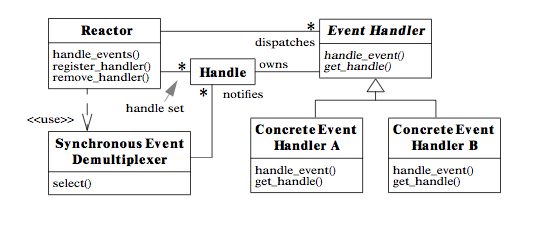
\includegraphics[width=12cm]{content/posa2/reactor/images/uml-diagram.png}
	\caption{Reactor UML-Diagramm}
\end{figure}



\begin{figure}[H]
	\centering
	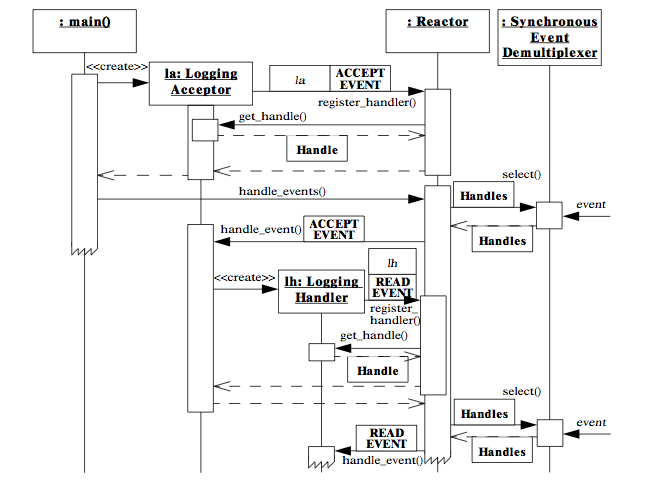
\includegraphics[width=12cm]{content/posa2/reactor/images/ssd.png}
	\caption{Reactor System sequence diagram}
\end{figure}


\subsection{Implementierung}

Die Implementierung des Reactors lässt sich in zwei Layer unterteilen. Der Frameworklayer, die die applikationsunabhängige demultiplex/dispatch Infrastruktur zur Verfügung stellt und der Applikationslayer, die die konkreten event handler liefert.


\subsection{Varianten}

\begin{itemize}
	\item \emph{Thread-Safe Reactor}
	\begin{itemize}
		\item Mit der normalen Variante ist Thread-Safety nicht nötig, da es das dispatchen der Hook Methods implizit innerhalb des Applikations-Prozesses macht
		\item Allerdings kann ein Reactor auch in multi-threaded applications benutzt werden
		\item Dort können mehrere Application Threads Event Handlers registrieren und entfernen
		\item u.a. Deshalb muss in diesem Fall ein Thread-Safe Reactor implementiert werden
	\end{itemize}
	\item \emph{Concurrent Event Handlers}
	\begin{itemize}
		\item Event Handlers laufen in dieser Variante in einem eigenen Thread
		\item Damit kann der Reactor indication events concurrently dispatchen
		\item Um das zu implementieren können folgende Patterns verwendet werden: Active Object, Leader/Followers, Half-Sync/Half-Async
	\end{itemize}
	\item Concurrent Synchronous Event Demultiplexer
	\begin{itemize}
		\item In der standard implementation wird der sync. event demultiplexer seriell gecalled.
		\item wenn dieser concurrent gecalled wird, kann eine operation auf einem Handle initiiert werden ohne dass die Operation geblockt wird
	\end{itemize}
\end{itemize}


\subsection{Verwendung}
\begin{itemize}
	\item libevent
	\item Apache Mina
	\item Node.js
	\item Vert.x
	\item Python Twisted
	\item Ruby EventMachine
\end{itemize}


\subsection{Vorteile}

\begin{itemize}
	\item klare Trennung von Framework- und Applikationslogik
	\item Modularität von event-gesteuerten Anwendungen durch verschiedene event handler
	\item Portabilität durch Trennung von Interface und Implementierung des Reactors
	\item einfache Parallelität durch den synchronen event demultiplexer
\end{itemize}


\subsection{Nachteile}

\begin{itemize}
	\item setzt einen event demultiplexer voraus
	\item Durchsatzprobleme bei lang laufenden event handler in single Threaded Applikation, dadurch, dass der event handler den Reactor blockiert
	\item schwierig zu testen durch die inversion of control (Don't call us, we call you)
\end{itemize}


\subsection{Prüfungsfragen}
\begin{itemize}
	\item Was ist der Unterschied zum Proactor?
	\begin{itemize}
		\item ...
	\end{itemize}
\end{itemize}